\documentclass{article}
\usepackage{tikz}
\usetikzlibrary{arrows.meta}

\begin{document}

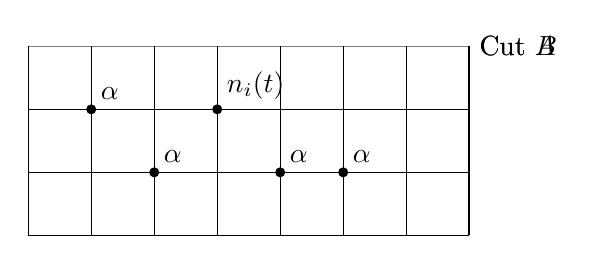
\begin{tikzpicture}[scale=0.8]
    % Draw the grid
    \draw[help lines] (0,0) grid (7,3);
    
    % Draw the vertical lines with labels
    \foreach \x in {0,1,...,6} {
        \draw (\x,0) -- (\x,3);
    }
    
    % Draw the horizontal lines with labels
    \foreach \y in {0,1,...,2} {
        \draw (0,\y) -- (7,\y);
    }
    
    % Draw the black dots
    \filldraw[black] (2,1) circle (2pt) node[above right] {$\alpha$};
    \filldraw[black] (4,1) circle (2pt) node[above right] {$\alpha$};
    \filldraw[black] (5,1) circle (2pt) node[above right] {$\alpha$};
    \filldraw[black] (3,2) circle (2pt) node[above right] {$n_i(t)$};
    \filldraw[black] (1,2) circle (2pt) node[above right] {$\alpha$};
    
    % Draw the vertical lines for the cuts
    \draw[thick] (7,0) -- (7,3) node[right] {Cut $A$};
    \draw[thick] (7,2) -- (7,3) node[right] {Cut $B$};
    
    % Draw the vertical line for the cut A
    \draw[thick] (7,0) -- (7,1);
    
    % Draw the vertical line for the cut B
    \draw[thick] (7,2) -- (7,3);
    
    % Draw the vertical line for the cut A
    \draw[thick] (7,1) -- (7,2);
    
\end{tikzpicture}

\end{document}